\subsection{Creating Bathymetries} \label{sec:bathys}
To facilitate the model a set of 14 bathymetries were created in $5$Ma time steps. These run from 65Ma to the present day configuration. These were reconstructed from bathymetries gained in \cite{Baatsen2016Aug}.
These bathymetries which were originaly $0.5^{\circ} \times0.5^{\circ}$, were subsequently scaled to a 4 degree model using Gaussian interpolation. Next, the land masks were manually edited to include passages and exclude some inland seas. Due to the low resolution of the model, choices have to be made with respect to the opening of certain passages. One of the choices that was made is that the northern Arctic sea is closed of in all of the bathymetrys. This is mainly due to the fact that 4 degree models do not have enough resolution to facilitate this sea and Veros lacking the ability to have polar flow.
The main events that shape the oceanic passages can be devided into time periods. These time periods are defined in \cref{tab:timeperiods}.
\begin{table}[H]
\centering
	\begin{tabular}{lll}
		&From &Until \\
		Paleocene & 65Ma&55Ma    \\
		Eocene    & 50Ma&35Ma     \\
		Oligocene & 30Ma&20Ma    \\
		Miocene   & 15Ma&Present 
	\end{tabular}
\caption{Time periods covered by this paper}
\label{tab:timeperiods}
\end{table}
The discussion on each time period is split. Here we address each of the periods and their respective changes.
\subsubsection{Paleocene}
In the Paleocene a vast Pacific exists almost serving as a single basin. This period is largely characterized by the growth and development of a larger atlantic basin. Subsequently a decrease in size of the pacific basin is also observed. The drake passage is explicitly chosen to be closed in this time period, there is some evidence of it being opened in the paleocene due to a major change in the motion of the South American and Antarctic plates until about 50Ma (\cite{Livermore2005Jul}). However, the evidence proposes a shallow opening of less than 1 km in depth. These uncertainties and the shallow nature of the opening has led to the decision to close the passage until its certain deep water connection starting after the late Eocene as also indicated by \cite{Livermore2005Jul}.

It is also of interest to note the existence of a range of islands between the Indian continent and the Eurasian continent which dissapears in this period.  These islands are called the Kohistan-Ladakh Arc (\cite{Jagoutz2009}). These may have had quite significant effect on the flow through the thetys seaway and are thus an interesting topic to discuss later on. 
\end{multicols}
%example full width overturning

\begin{figure}[H]
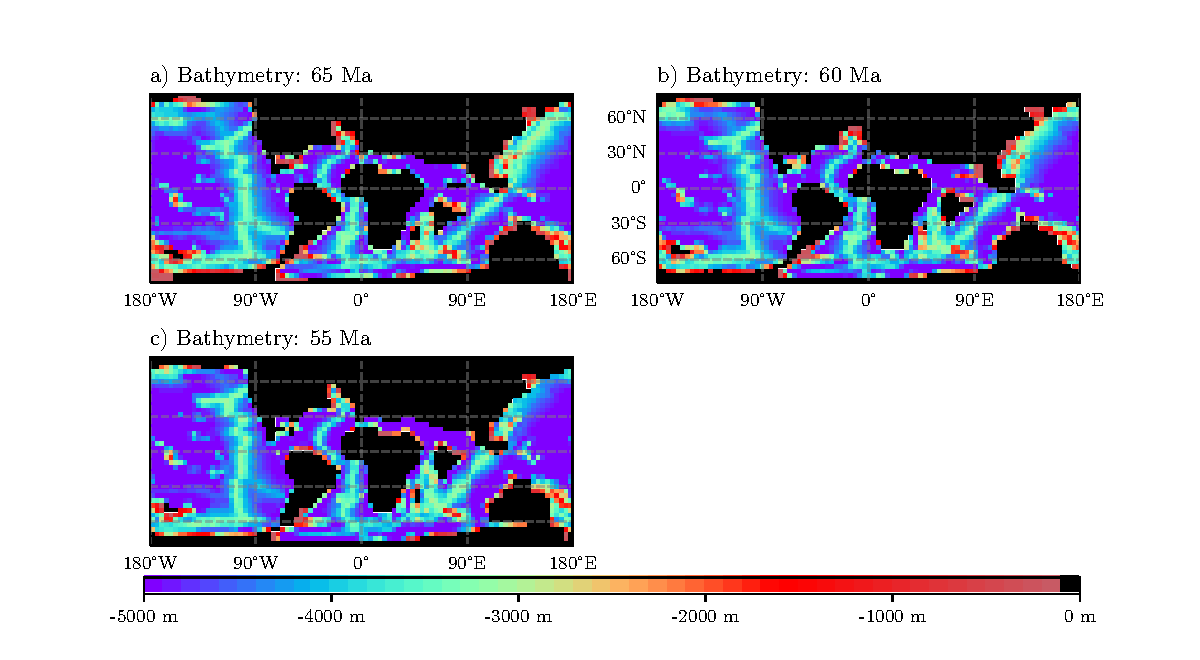
\includegraphics[width=\linewidth]{bathymetries_paleocene.pdf}
\caption{Paleocene Bathymetries showing \textbf{(a)} The bathymetry of 65 Ma. \textbf{(b)} The bathymetry of 60 Ma. \textbf{(c)} The bathymetry of 55 Ma}
\end{figure}
\begin{figure}[H]
	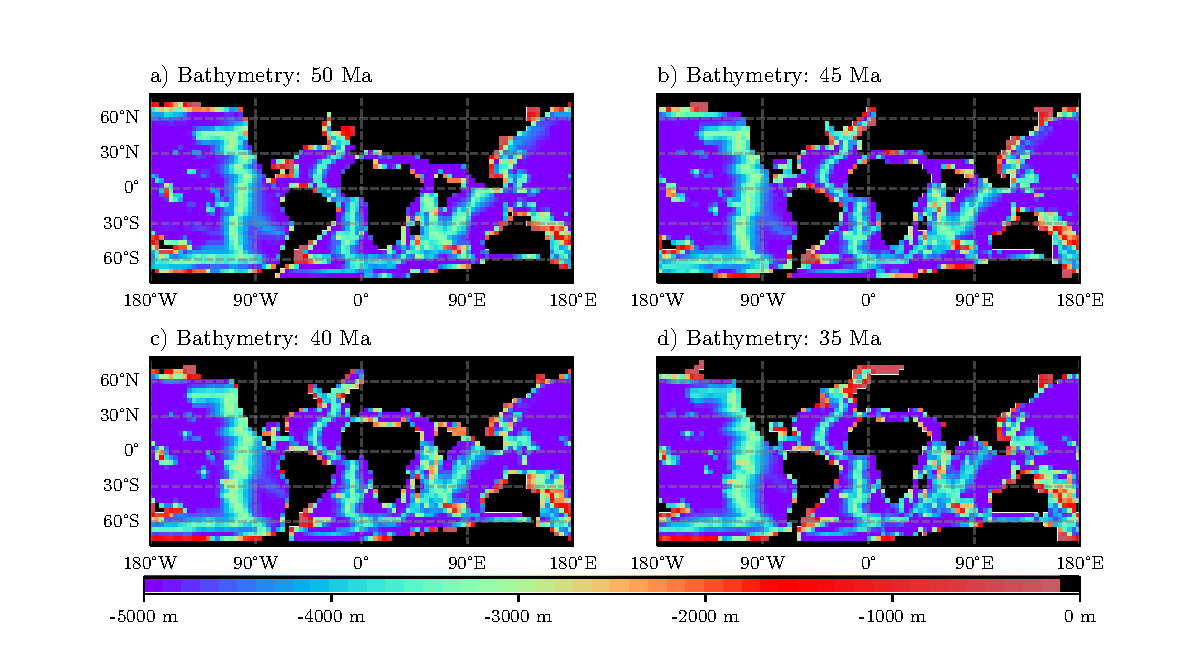
\includegraphics[width=\linewidth]{bathymetries_eocene.pdf}
	\caption{Eocene Bathymetries showing \textbf{(a)} The bathymetry of 50 Ma. \textbf{(b)} The bathymetry of 45 Ma. \textbf{(c)} The bathymetry of 40 Ma.\textbf{(d)} The bathymetry of 35 Ma}
\end{figure}

\begin{multicols}{2}
\subsubsection{Eocene}
The Eocene in contrast to the Paleocene is distinguished by the opening of certain passages connecting oceanic basins. These effects are often studied extensively for each individual passage in literature. Choosing the exact timing for opening the passages is done manually by looking at often active research. The first of such passages to open is the Tasman passage which is opened at 35Ma as a shallow passage slowly growing in size(\cite{Lawver2003Sep}). The Tasman passage opening is believed to have had a large impact on the onset of the Atlantic circumpolar current (ACC). Some authors even suggests its influence on the onset of a early "proto-ACC" (\cite{Sarkar2019Jul}). This proto-ACC may have caused upwelling of northern-sourced nutrient-rich deep equatorial Pacific waters in the south Pacific. However, this is assuming an open drake passage, which does not exist in our bathymetries. Thus, this upwelling will likely not be observed until the early Oligocene. 

From the onset of the early Eogene the Indian Continent has been fast moving towards the north slowly closing the northern passage between the Indian ocean and the Tethys seaway. The deep water passage is closed from 35Ma based onwards \cite{Najman2010Dec}. This limits the throughflow through the Thetys seaway to purely east of the Indian continent. Which is now in effect part of the larger Eurasian continent. 

\subsubsection{Oligocene}
From the onset of the Oligocene The Total circulation of water around the Antarctic basin is finalized by the opening of the shallow Drake passage at around 30Ma. 30Ma is specifically chosen to differentiate between the opening of the drake and Tasman passages. Especially since there is still some debate on the exact timing of drake passage opening (\cite{Scher2006Apr}; \cite{Livermore2005Jul}). These openings coincide with the onset of the ACC that has had major effects on the global climate variability. Furthermore, The Oligocene is characterized by the further expansion of the Atlantic basin and a shallower Thetys seaway. Furthermore a deep water area starts existing between what is now Greenland and the European continent. This water basin is now known to be central to the deep water formations of the northern Atlantic.
\end{multicols}
%example full width overturning

\begin{figure}[H]
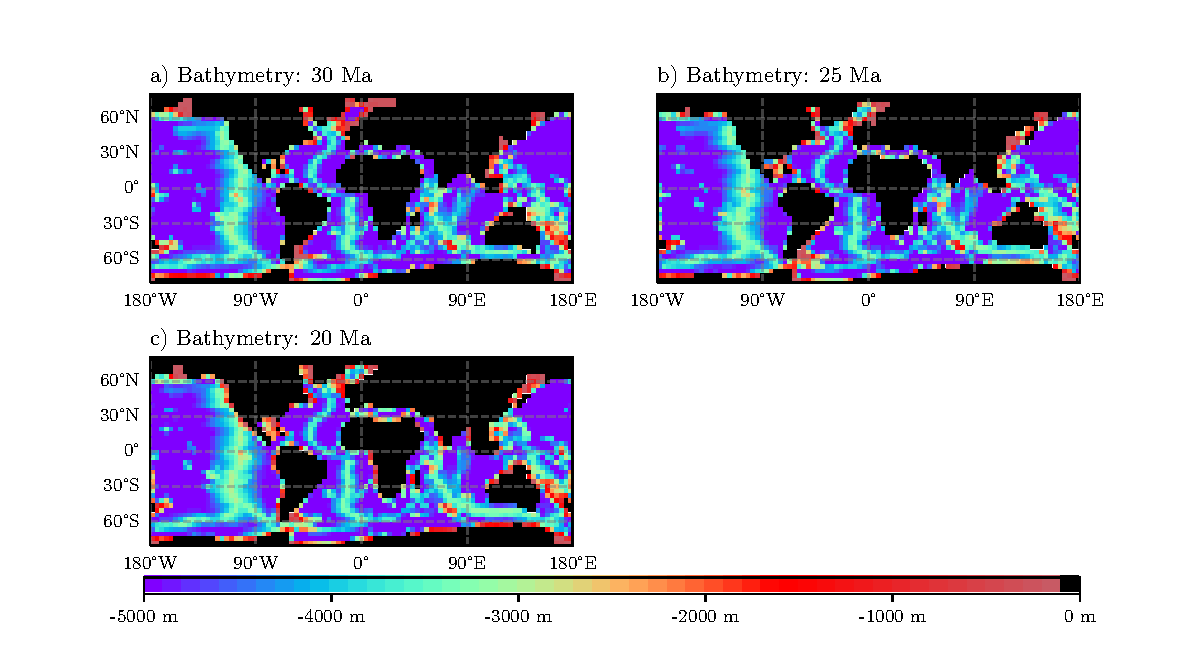
\includegraphics[width=\linewidth]{bathymetries_oligocene.pdf}
\caption{Oligocene bathymetries showing: \textbf{(a)} The bathymetry of 30 Ma. \textbf{(b)} The bathymetry of 25 Ma. \textbf{(c)} The bathymetry of 20 Ma.}
\end{figure}
\begin{figure}[H]
	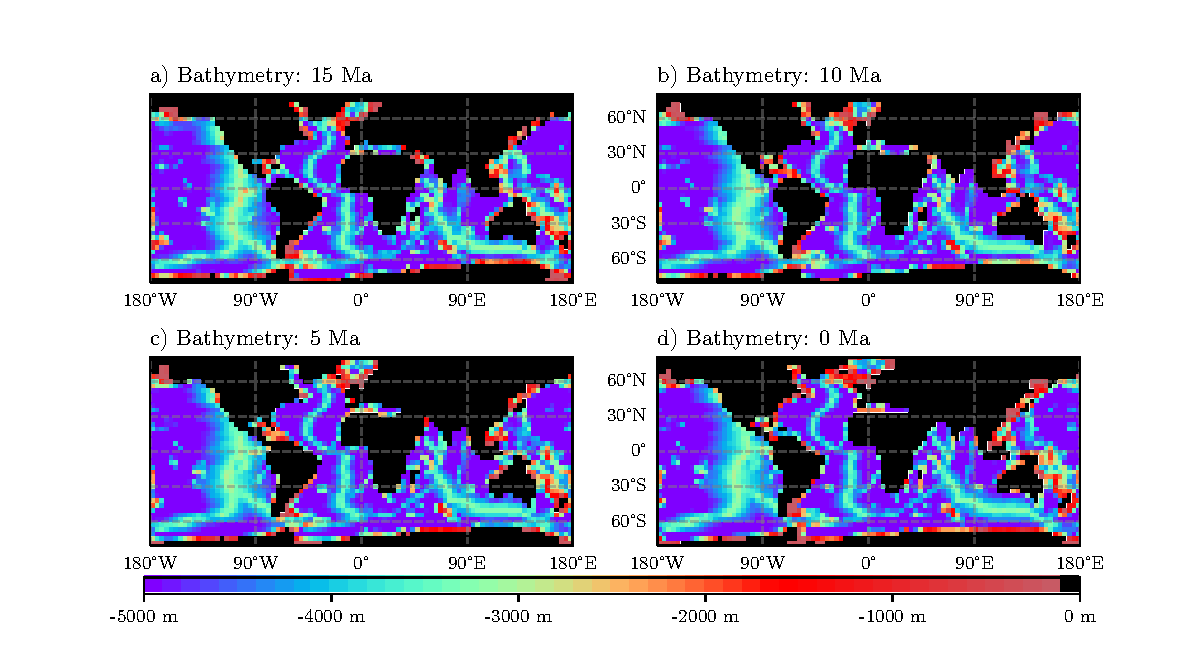
\includegraphics[width=\linewidth]{bathymetries_miocene.pdf}
	\caption{Miocene bathymetries showing \textbf{(a)} The bathymetry of 15 Ma. \textbf{(b)} The bathymetry of 10 Ma. \textbf{(c)} The bathymetry of 5 Ma.\textbf{(d)} The present day bathymetry}
\end{figure}

\begin{multicols}{2}
\subsubsection{Miocene}
Finaly, the Miocene is Characterized by Some more passage closures. The Tethys seaway had been decreasing in size for the duration of our bathymetries. It finally fully detaches the mediteranian sea from the Indian ocean from 15Ma onward(\cite{Hamon2013Nov}). Then another major change occurs with the closure of the panama seaway from 5Ma onward  (\cite{Molnar2008Jun}; \cite{Pindell1988Dec}). Stopping the mid latitude throughflow between the Atlantic and Pacific basins. The throughflow in the panama seaway is believed is believed to have reversed in direction with the onset of the decrease in size and subsequent closure of the Thetys ocean (\cite{von2006effect}; \cite{omta2003physical}). Something that will be studied more closely in the discussion of our results.

